\documentclass{MScthesisITEM}

% this package is just to generate text for demo-purposes
\usepackage{blindtext}


\title{Visual Sensing in Mobile Robots} % The title of your assignement; NB use \newlinetitle to start a newline
\author{Vegard S. Lindrup} % Your firstname and lastname
\professor{Firstname Lastname, Affiliation} % Affiliation = ITEM for instance
\supervisor{Firstname Lastname, Affiliation}

%% Uncomment the following in case you want subfigures; note that there will be a warning for the caption package
% \let\subcaption\undefined
% \let\subfloat\undefined
% \usepackage[bf]{caption}
% \usepackage{subcaption}

\DeclareGraphicsExtensions{.pdf,.jpg,.png}
\graphicspath{{./figs/}}
\usepackage{subcaption}

\loadglsentries{glossary}
\makeglossaries

\begin{document}
\selectlanguage{english}
\pagenumbering{roman}
\pagestyle{plain}

%% Only for the project; comment out the line below for the master's thesis; the front page will be generated automatically by DAIM
\titleITEM

%% Only for the master's thesis; for the project report the description is taken from It's Learning and added by the department
% \selectlanguage{english} % Change to 'norsk' if you are writing in Norwegian
% \begin{titlingpage}

\noindent
\begin{tabular}{@{}p{4cm}l}
\textbf{Title:} 	& \thetitle \\
\textbf{Student:}	& \theauthor \\
\end{tabular}

%\vspace{4ex}
%\noindent\textbf{Problem description:}
%\vspace{2ex}

\section*{Problem description}

\subsection*{Introduction}

This project is a continuation of previous projects in developing a concept for robotic maintenance performed by a mobile autonomous robot.  Over the course of previous projects, the system has been equipped with a robot manipulator arm, several sensors, a wireless router, on-board power supply based on batteries and a central PC. This equipment is mounted on a steel wagon. The wagon stands on four omni-wheels, each with their own electric motor drivers.

\subsection*{Project Goals}

To increase the robot`s degree of autonomy, it is desired to explore possibilities for reliable and safe movement of the robot without involving a person. The purpose of such a movement may be to reach a docking station or a location where a maintenance or an inspection task will be performed while avoiding obstructions and hazardous situations. As a step towards achieving these goals, the following points shall be carried out:

\begin{enumerate}
	
	\item Explore potential methods for autonomous navigation that may fulfill the goals above, where computer vision is the primary navigational aid. 
	
	\item Implement one, several or a combination of the methods found in point one. This includes selection and installation of new equipment, e.g. cameras, if necessary. 
	
	\item Performance and suitability assessment of the selected implementation with respect to autonomous navigation.
	
	\item Assess how well the system handles errors and potentially hazardous states and situations.
	
	\item Propose changes to the implementation and suggest further work in order to improve the safety and reliability of the system and its ability to navigate autonomously.

	
\end{enumerate}
\vspace{6ex}

\noindent
\begin{tabular}{@{}p{4cm}l}
%\textbf{Responsible professor:} 	& \theprofessor \\
\textbf{Supervisor:}			& \thesupervisor \\
\end{tabular}

\end{titlingpage}
% \cleardoublepage

%% There must be an abstract in English, even though the main text is in Norwegian
\selectlanguage{english}
\pagestyle{empty}
\begin{abstract}
	\noindent \Blindtext[5][1]
\end{abstract}
\cleardoublepage

%% Only for the master's thesis; if the main text is in English and you can write Norwegian, there must be an abstract in Norwegian as well.
% \selectlanguage{norsk}
% \pagestyle{empty}
\renewcommand{\abstractname}{Sammendrag}
\begin{abstract}
\noindent Sikkerheten til nesten all offentlig nøkkel-kryptografi er basert på et vanskelig beregnbarhetsproblem. Mest velkjent er problemene med å faktorisere heltall i sine primtallsfaktorer, og å beregne diskrete logaritmer i endelige sykliske grupper. I de to siste tiårene, har det imidlertid dukket opp en rekke andre offentlig nøkkel-systemer, som baserer sin sikkerhet på helt andre type problemer. Et lovende forslag, er å basere sikkerheten på vanskeligheten av å løse store likningsett av flervariable polynomlikninger. En stor utfordring ved å designe slike offentlig nøkkel-systemer, er å integrere en effektiv ``falluke'' (trapdoor) inn i likningssettet. En ny tilnærming til dette problemet ble nylig foreslått av Gligoroski m.f., hvor de benytter konseptet om kvasigruppe-strengtransformasjoner (quasigroup string transformations). I denne masteroppgaven beskriver vi en metodikk for å identifisere sterke og svake nøkler i det nylig foreslåtte multivariable offentlig nøkkel-signatursystemet MQQ-SIG, som er basert på denne idéen.

Vi har gjennomført et stort antall eksperimenter, basert på Gröbner basis angrep, for å klassifisere de ulike parametrene som bestemmer nøklene i MQQ-SIG. Våre funn viser at det er store forskjeller i viktigheten av disse parametrene. Metodikken består i en klassifisering av de forskjellige parametrene i systemet, i tillegg til en innføring av konkrete kriterier for hvilke nøkler som bør velges. Videre, har vi identifisert et unødvendig krav i den originale spesifikasjonen, som krevde at kvasigruppene måtte oppfylle et bestemt kriterie. Ved å fjerne denne betingelsen, kan nøkkel-genererings-algoritmen potensielt øke ytelsen med en stor faktor. Basert på alt dette, foreslår vi en ny og forbedret nøkkel-genereringsalgoritme for MQQ-SIG, som vil generere sterkere nøkler og være mer effektiv enn den originale nøkkel-genereringsalgoritmen.  
\end{abstract}
% \cleardoublepage

\selectlanguage{english}% Change to 'norsk' if you are writing in Norwegian

\renewcommand{\abstractname}{Preface}
\begin{abstract}
\noindent \blindtext 
\end{abstract}
%\cleardoublepage

%% include if relevant
\listoffigures
\clearpage
	%\cleardoublepage
	
%% include if relevant
\listoftables
\clearpage
%\cleardoublepage
	
%% include if relevant
%\listofalgorithms
%\addcontentsline{toc}{chapter}{List of Algorithms}
%\cleardoublepage
	
%% include if relevant
\printglossary[title=List of Symbols, style=long]
%\cleardoublepage
\glsaddall[]
	
%% include if relevant
\printglossary[title=List of Acronyms,type=\acronymtype] % prints just the list of acronyms
%\cleardoublepage

% similarly you may add a separate acknowledgments page

\tableofcontents*
\clearpage
%\cleardoublepage

\pagenumbering{arabic}
\pagestyle{ruled}
\chapter{Introduction}
\label{chp:introduction} 

This section is intended to provide an overview of the contents and context of this report. The first part of this section gives a brief introduction to the field of mobile autonomous robotics and computer vision, as well as the benifits and potential applications for this technology. The robot system and tools used in the project is presented in subsection \ref{}. Lastly, each of the following sections will given short introductions.




\section{Mobile Autonomous Robotics and Computer Vision}

Put the task into a larger context. Bring in some points on the societal impact of autonomous robotics and the increased potential of mobile robotics.  

The field of computer vision has seen an enormous growth over the last few decades - not only in scale, but in accessibility and capability as well. As a consequence of this recent growth, tapping into the field of computer vision is bound to reveal applications that are useful for a mobile autonomous maintenance robot. Recent discoveries within computer vision includes robust feature recognition and object detection, face detection and video processing. The latest great additions to the field are Big Data and Artificial Intelligence.

\section{System Overview}

The mobile robot being worked on in this project is shown in figure \ref{fig:RobotFront}. The manipulator arm  has been used in previous projects on robotic maintenance, and it was placed on the mobile platform during the master thesis of (Aspunvik og siter). This section provides a short description of the hardware. If a more detailed description of the robot and it's equipment is required, consult the thesis of Aspunvik[cite]. 

\begin{figure}
\centering
 \begin{subfigure}[b]{0.3\textwidth}
        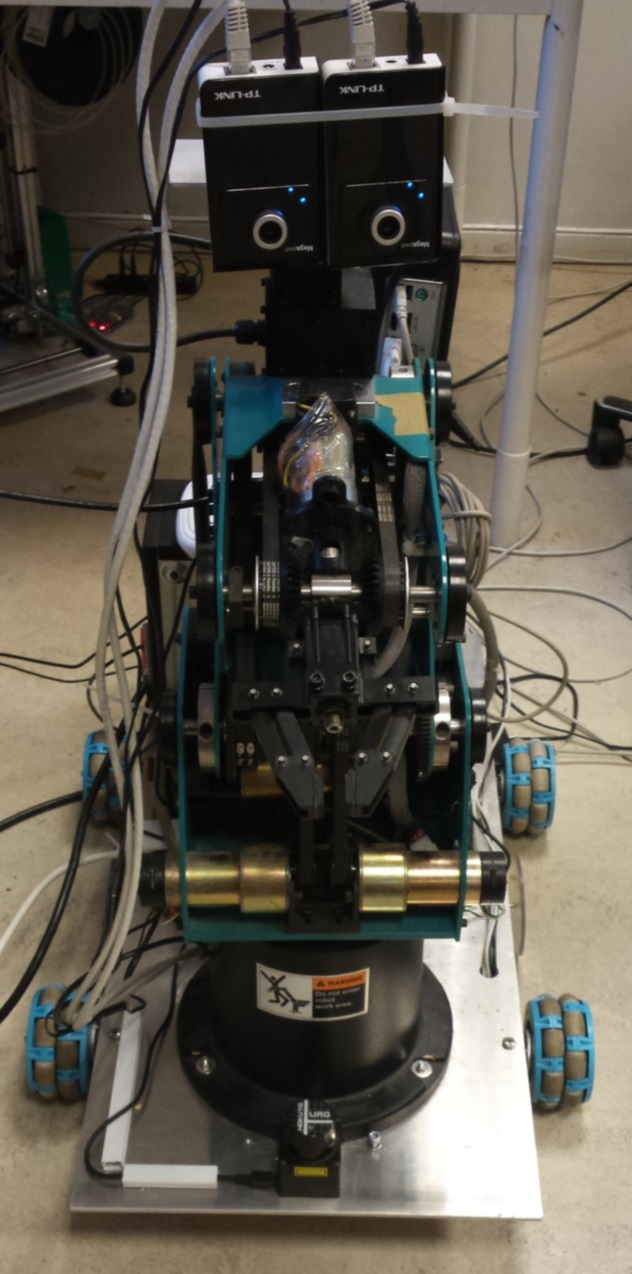
\includegraphics[width=\textwidth]{Robot_front}
        \caption{Front view.}
        \label{fig:RobotFront}
    \end{subfigure}
    \begin{subfigure}[b]{0.65\textwidth}
        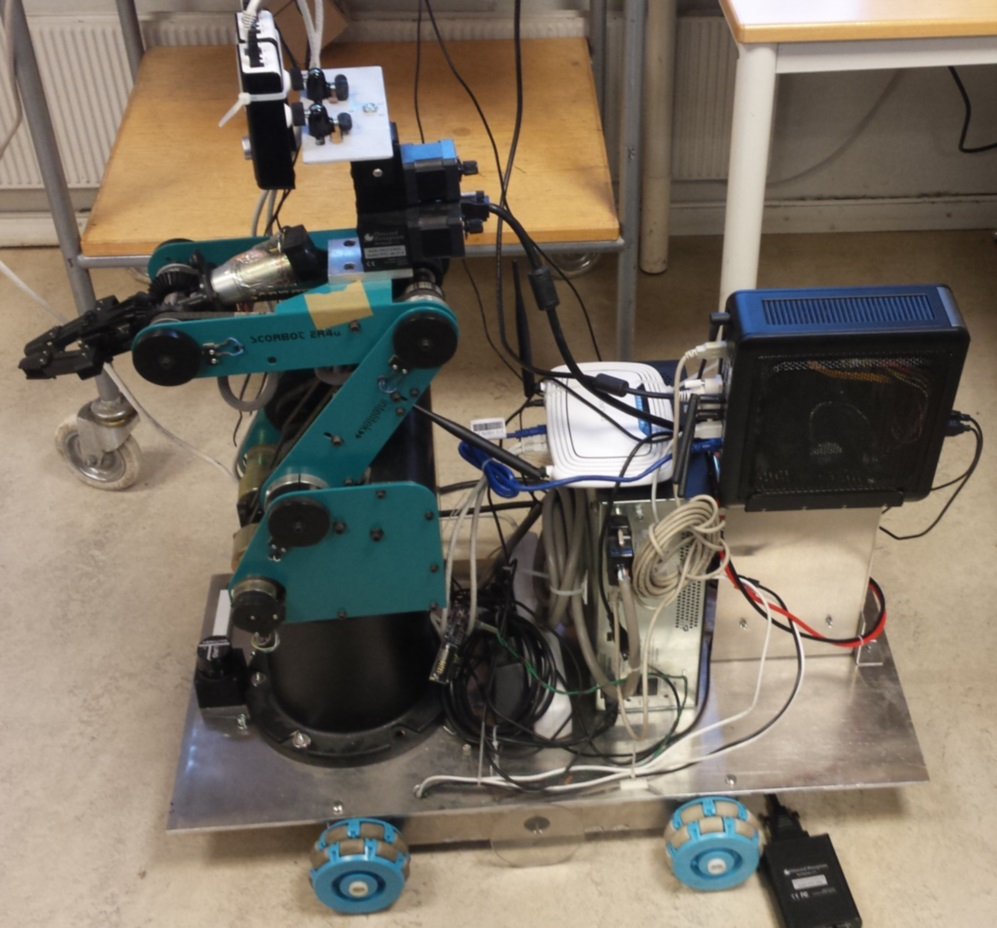
\includegraphics[width=\textwidth]{Robot_side}
        \caption{Side view.}
        \label{fig:RobotSide}
    \end{subfigure}
    \caption{\label{fig:RobotView}The robot used in the project.}
\end{figure}

\subsection{Propulsion}

The steel chassis of the robot stands upon four omni-wheels. The wheel pairs are placed in parallel, making the vehicle uncontrollable along the lateral axis. Each wheel is powered by an electrical motor and motor driver. The motor drivers are controlled with pulse width modulation by an evaluation board from Atmel,(atmel kort).  

\subsection{Sensors}

The robot was outfitted with several sensors over the course of previous projects. These are:
\begin{itemize}
	\item Two odometer wheels with encoders. One on each side. 
	\item Two infrared distance sensors. 
	\item A LIDAR (Light Detection and Ranging).
	\item Two IP-cameras.
\end{itemize} 

Only the cameras were used in this projects. 

\subsection{The Manipulator}

\begin{figure}
	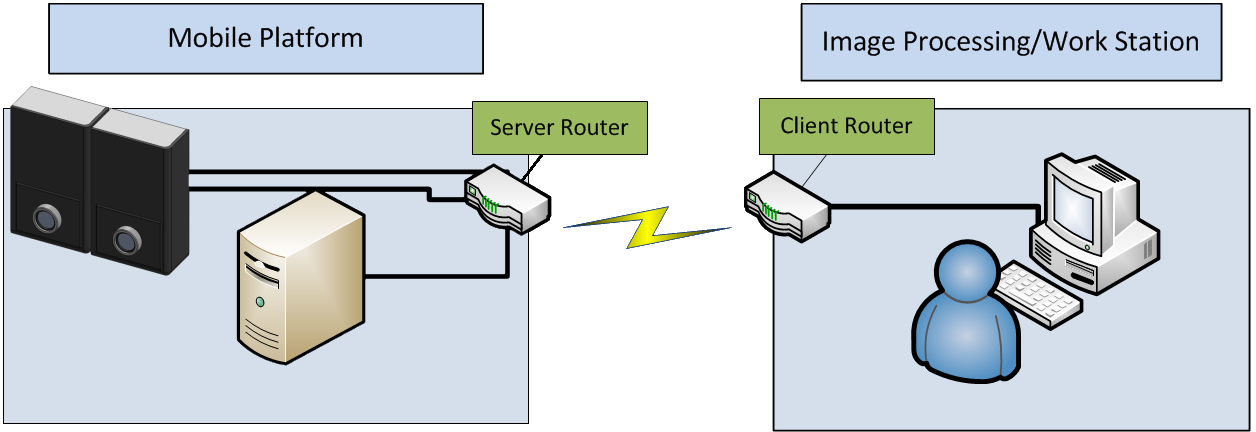
\includegraphics[width=1\textwidth]{hardwareSetup_cropped}
\end{figure}

\section{Report Structure}
How the report is structured, and a very brief description of the contents in each section.
%% include here the other chapters
\chapter{Background Theory}\label{chp:theory}

\section{Introduction to Computer Vision}

\subsection{Introduction}
This chapter contains the background theory which is necessary to understand the implementations in chapter \ref{chp:implementation} and how they are intended to work. 

\subsection{How it's Done}
nanana

\subsection{OpenCV}

OpenCV (Open Source Computer Vision Library) is an  open source library with a vast number of advanced computer vision and machine learning algorithms. The library supports Windows, Linux, iOS and Android, and has interfaces to C, C++, Python, Java and MATLAB. All OpenCV applications in this project uses OpenCV 3.0.0 for Windows. OpenCV for Windows can be downloaded from sourceforge.net. This download contains source files, sample programs, sample data and a pre-built library for MSVC 2010 and 2013. The pre-build library can quickly be plugged into  an IDE such as Qt Creator or Visual Studio 2013, thus giving the programmer access to all basic OpenCV features. A steb-by-step guide for using both the pre-built and a custom-built library can be found in Appendix \ref{chp:setup}.

\begin{figure}
\centering
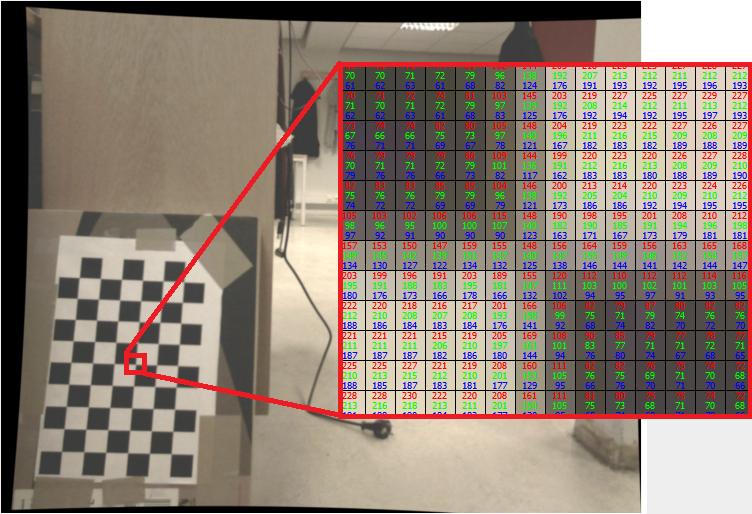
\includegraphics[scale=0.7]{SjakkMat}
\caption{Elements in a cv::Mat representing an image. This is a 3-channel image with 8 bit RGB colors.}
\label{fig:matGrid}
\end{figure}

\section{Stereo Vision and Depth Perception}

Stereo vision and depth perception is one of the core topics within this report. Here, the theory behind a method using two cameras is presented, while some additional methods are mentioned to provide context. 

\subsection{Various Methods}

Methods for depth perception in computer vision can be separated into two main categories, i.e. active and passive. Active sensors will usually project a light pattern onto the scene to be perceived, before sensing how this pattern is displaced by the topology of the scene. The Kinect sensor and 3d-scanners using laser light are typical examples of active sensors. Passive depth perception makes use of many of the same cues we use to perceive depth. The most common passive sensors extract the depth information by observing observing a scene from at least two different positions. 

Optical flow is another important method for depth perception. Optical flow may be either active or passive. The passive variant requires  only one camera, but depends on motion and a stream of images to extract depth information. Observing how much some chosen features in a scene has moved in the image frame at $t = 1$ compared to the frame at $t = 0$ is the basis of depth sensing from optical flow. When the camera moves through a scene where all objects are stationary, objects that are far away will naturally have an optical flow field with a smaller magnitude than objects that are close. 

\subsection{Stereoscopic Vision in General}

In this project, passive stereoscopic vision is achieved by using two identical (in theory) cameras placed on the same plane. The gist of passive stereoscopic vision is based on the fact that objects close to the camera pair will have a large displacement from the left to the right camera compared to objects that are further away. This concept is illustrated in figure \ref{fig:3dScene}.

\begin{figure}
\centering
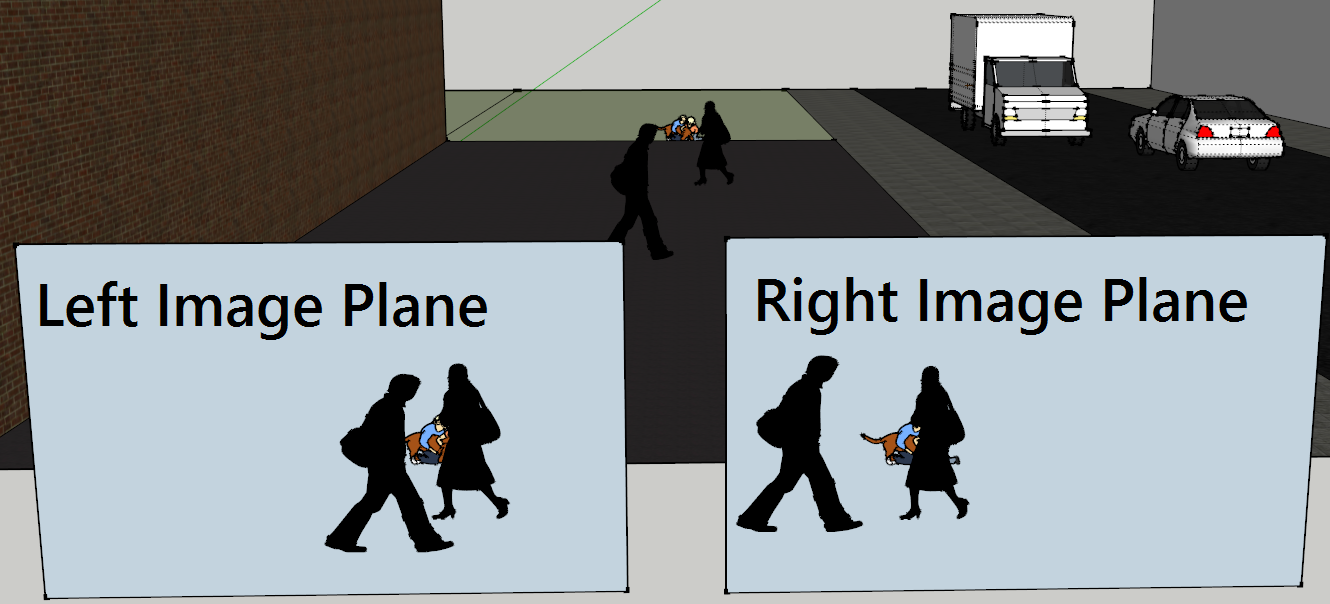
\includegraphics[scale=0.4]{3dScene}
\caption{\label{fig:3dScene}Left to right displacement on the image plane based on distance.}
\end{figure} 

\paragraph{The Pinhole Camera Model}

Figure \ref{fig:pinhole} illustrates the geometry of a pinhole camera. In a pinhole camera, a scene will be projected onto an image plane, often denoted $\pi$, through the camera projection point $O$ which is located at the origin. The focal length $f$ is the distance from the projection point $O$ to the image plane $\pi$. In a true pinhole camera the image plane will be located behind the lens and the projection point $O$, and the scene projection will be rotated by $180^{\circ}$. A virtual image plane placed in front of $O$ is intended to make the figure more straightforward. 

\begin{wrapfigure}{r}{0.6\textwidth}
    \vspace{-10pt} % Remove exessive whitespace
    \centering
    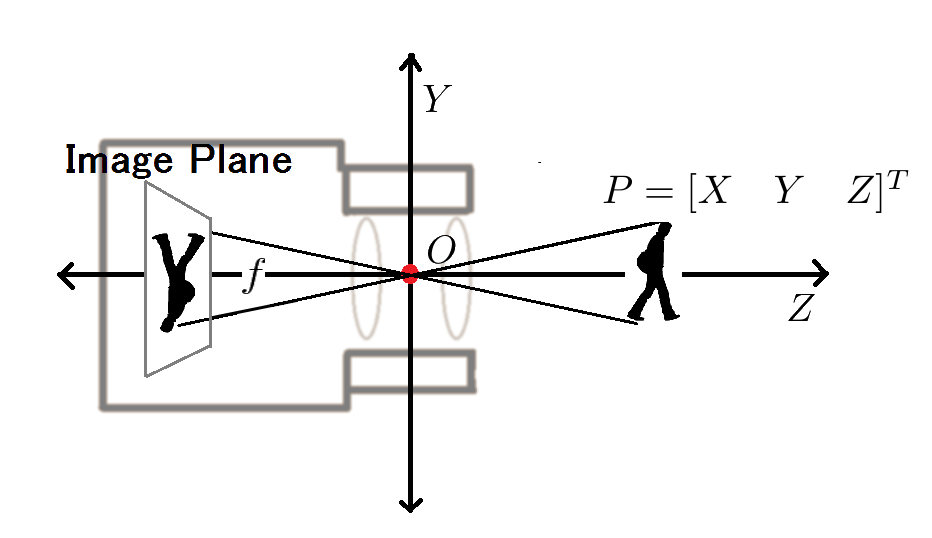
\includegraphics[width=0.6\textwidth]{pinhole}
    \caption{\label{fig:pinhole}Geometry of a pinhole camera.}
    \vspace{-10pt} % Remove exessive whitespace
    \label{phantompic}
\end{wrapfigure}

\paragraph{Stereo Cameras}

Figure \ref{fig:StereoSpace} shows an ideal stereo camera model.  The model comprise two pinhole camera models where the virtual image planes are located on the same plane. The two image planes are separated by a horizontal translation $B$ which is called the baseline. This implies that the projection point $O_L$  in the left camera, relates to the projection point $O_R$ on the right camera through $B$: $O_R = O_L + B$. Each of the two image planes has a left handed pixel based coordinate system $u,v$, i.e. the origin is in the top left corner and the opposite pixel is in the bottom right corner. 

\begin{figure}
\centering
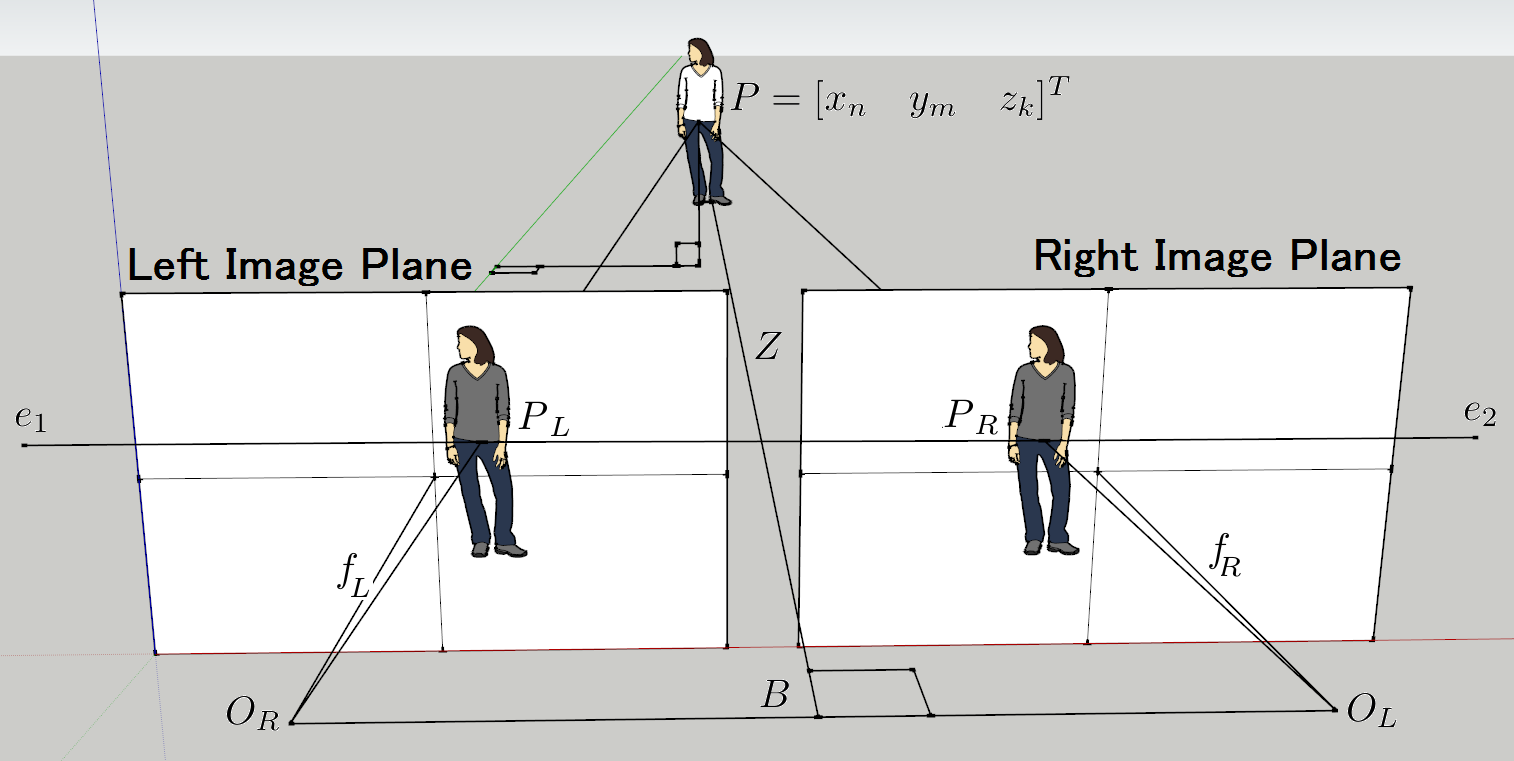
\includegraphics[width=1\textwidth]{StereoSpace}
\caption{\label{fig:StereoSpace}Geometry of stereo vision.}
\end{figure}

\paragraph{Camera Distortion}

A downside of the otherwise cheap and useful pinhole camera is camera distortion. The distortion is usually severe enough to render the camera useless as a sensor if it is not calibrated. Calibration in OpenCV accounts for radial and tangential distortion by finding five distortion coefficients \cite{3dCalib}:

%\vspace{-1em}
\begin{equation*}
	 Distortion_{coefficients} = (k_1 \quad k_2 \quad p_1 \quad p_2 \quad k_3)
\end{equation*}
%\vspace{-0.2em}
\textbf{where} 
%\vspace{-1.1em}
\begin{equation*}
 	p_i \quad with \quad i \in \left\{1, 2\right\}
\end{equation*}
%\vspace{-0.3em}
\textbf{are the radial distortion constants, and}
%\vspace{-0.2em}
\begin{equation*}
	k_i \quad \textrm{with} \quad i \in \left\{1, 2, 3\right\}  
\end{equation*}
%\vspace{-0.5em}
\textbf{are the tangential distortion constants.} 
%\vspace{-0.5em}

\subsection{Stereoscopic Vision in OpenCV}

The prebuilt version of OpenCV 3.0.0 comes with two stereo matching algorithms: \gls{bm} Block Matching (StereoBM) and Semi Global Block Matching (StereoSGBM). Additional algorithms are available if OpenCV is built with, e.g. CUDA.

\paragraph{StereoSGBM}\cite{hirschmullerstereo}
blablabalb \gls{bm}.

\chapter{Example}
\label{chp:example} 

Here is an example of how to use acronyms such as \gls{ntnu}. The second time only \gls{ntnu} is shown and if there were several you would write \glspl{ntnu}. And here is an example\footnote{A footnote} of citation~\cite{Author:year:XYZ}. 

\Blindtext[3][1]

\begin{figure}
\centering
% dummy figure replacement 
\begin{tabular}{@{}c@{}}
\rule{.5\textwidth}{.5\textwidth} \\
\end{tabular}
\caption{\label{fig:example}A figure}
\end{figure}

\section{First section}\label{sec:first_section}

\subsection{First subsection with some \texorpdfstring{$\mathcal{M}ath$}{Math} symbol}\label{sec:first_ssection}

\blindtext
\begin{itemize}[topsep=-1em,parsep=0em,itemsep=0em] % see http://mirror.ctan.org/macros/latex/contrib/enumitem/enumitem.pdf for details about the parameters
 \item item1
 \item item2
 \item ...
\end{itemize}

\subsection{Mathematics}

\blindmathtrue
\blindtext

$B$ \\
$X_L$\\
$X_R$\\
$P_R$\`\
$P_L$\\
$P = [X \quad Y \quad Z]^T$\\
$P = [x_n \quad y_m \quad z_k]^T$\\
$e_1$\\
$e_2$\\
$O_R$\\
$O_L$\\
$X = [x \quad y \quad z]^T$\\
$f$\\
$Z$\\
$Y$\\
$VP$\\
$Hz$


\begin{proposition}\label{def:a_proposition}
A proposition... (similar environments include: theorem, corrolary, conjecture, lemma)

\end{proposition}

\begin{proof}
\vspace*{-1em} % Adjust the space when parskip is set to 1em
And its proof.
\end{proof}

\begin{table}
\caption{\label{tab:example}A table}
\centering
\begin{tabular}[b]{| c | c | c | c | c |}
\hline
a & b & c & d & e \\ \hline
f & g & h & i & j \\ \hline
k & l & m & n & o \\ \hline
p & q & r & s & t \\ \hline
u & v & w & x & y \\ \hline
z & æ & ø & å &   \\ \hline
\end{tabular} 
\end{table}

\subsection{Source code example}

% \floatname{algorithm}{Source code} % if you want to rename 'Algorithm' to 'Source code'
\begin{algorithm}[h]
  \caption{The Hello World! program in Java.}
  \label{hello_world}
  % alternatively you may use algorithmic, or lstlisting from the listings package
  \begin{verbatim}
  
class HelloWorldApp {
  public static void main(String[] args) {
    //Display the string
    System.out.println("Hello World!");
  }
}
\end{verbatim}
\end{algorithm}

You can refer to figures using the predefined command like \fref{fig:example}, to pages like \pref{fig:example}, to tables like \tref{tab:example}, to chapters like \Cref{chp:example} and to sections like \Sref{sec:first_section} and you may define similar commands to refer to proposition, algorithms etc.

\chapter{Implementation}\label{chp:implementation}

\section{Introduction}

An obstruction detector and a vanishing point detector are the two attempted implementations presented in this report. The obstruction detector uses stereo vision to perceive depth and distance to possible objects in the path of the robot. The vanishing point detector attempts to find a single vanishing point by detecting lines in the environment before selecting a vanishing point based on line intersections. 

\section{Vanishing Point Detection}

\subsection{Overview}

The goal of the vanishing point detector is to provide a setpoint for the robot to steer towards. In other words, steering towards a vanishing point is a good way to reach the end of a hallway or corridor. This was considered to be a good starting point, and possible expantions could be added later. Choosing a method as a basis for a vanishing point detector was not easy. The selected method should be simple, suitable for \gls{opencv} and not go too far beyond the prior knowledge of the author. Another important factor was that spending too much time on this implementation would come at the expense of the obstruction detector. A vanishing point detector method by D. Gerogiannis et. al. \cite{gerogiannisvp} showed promise as it was based on line detection, which has good support in OpenCV. The method in \cite{gerogiannisvp} appears to be suitable for structured environments with many straight lines, such as hallways, streets and corridors. The steps in the detection procedure are:

\begin{enumerate}
	\item Detect edges in the image, e.g. by using Canny edge detection.
	\item Detect line segments that may be used as vanishing lines based on edges found in step 1. Could be done with the Hough line transform.
	\item Filter the detected lines. This is done by modelling new lines by using the major axis of ellipses with very high eccentricity. The ellipses are generated by a split-and-merge algorithm. In short, it will merge similar line segments by assuming that their end points are collinear.
	\item Find line intersection points based on the new filtered lines. Each point is stored and assigned a weight.
	\item Find the vanishing point among the line intersections based on a voting scheme. 
\end{enumerate}

\subsection{Line Detection}

Line detection comprise step 1 and 2 from the list above. OpenCV comes with an implementation of the Canny edge detector ready for use. The detector returns a binary image of the detected edges. Edges are detected by convolving the input image with two kernels $G_x$ and $G_y$. The convolutions will indicate change gradients in the $x$ and $y$ directions which in turn will give the direction of a potential edge. Finally, the detector rejects or accepts potential edges based on two gradient thresholds. Gradients below the lower threshold are rejected, edges above the upper threshold are accepted, and edges between the thresholds are only accepted if their neighbouring gradients are above the upper threshold\cite{cannyedge}. 

\begin{wrapfigure}{r}{0.55\textwidth}
	\vspace{-10pt} % Remove exessive whitespace
	\centering
	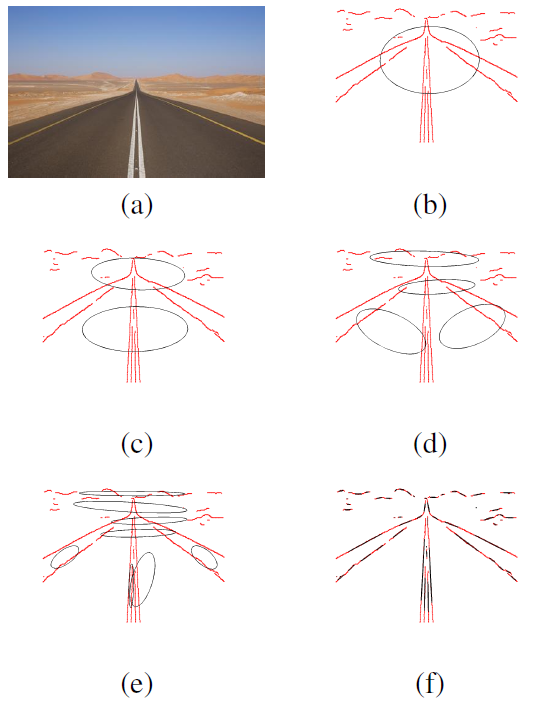
\includegraphics[width=0.6\textwidth]{GerogiannisLines}
	\caption{\label{fig:GerogiannisLines}Gerogiannis concept of representing lines by eccentric ellipses. This image is taken directly from \cite{gerogiannisvp}.}
	\vspace{-60pt} % Remove exessive whitespace
\end{wrapfigure}

At this point, we only have a simple binary image where edges are represented as white pixels on a black background. The next step is to interpret these edges as lines. Line detection is performed by using the probabilistic Hough line transform. This is an already implemented function, which takes in the edge image from the previous step, and return a set of point pairs representing line segments. The benefit of using the probabilistic detector is that it can perceive an edge with a discontinuity as a singe line. 

\subsection{Line Filtering}

Line filtering is performed by splitting and merging ellipses until their major axis represents a set of approximations to collinear points. The points is the set of points that define the previously detected line segments. This algorithm is called \gls{dsam}, and it is explained in another paper by D. Gerogiannis \cite{gerogiannisshape}. Line segments returned from the probabilistic Hough transform will often overlap or be very close to each other. The purpose of this step is to get a cleaner representation of the contours in the environment.

Figure \ref{fig:GerogiannisLines}, taken from \cite{gerogiannisvp}, illustrates the steps in the \gls{dsam} algorithm.

\subsection{Vanishing Point Detection}

\begin{wrapfigure}{r}{0.35\textwidth}
	\vspace{-10pt} % Remove exessive whitespace
	\centering
	\includegraphics[width=0.36\textwidth]{getVp}
	\caption{\label{fig:getVp}Two steps in "getVanishingPoint()".}
	\vspace{-60pt} % Remove exessive whitespace
\end{wrapfigure}


When the detected lines have been filtered and stored, they will be passed to the vanishing point detector in the function "getVanishingPoint(lines)". This function will perform two steps (figure \ref{alg:getVp}):

\begin{enumerate}
	\item Find, store and assign weights to the points where the lines intersect. Lines that are either too vertical or too horizintal will not be included in the calculations. Intersectionpoints outside the image frame are rejected.
	\item Find the vanishing point based on the valid weighted intersection points. This is done by a voting scheme described in \cite{gerogiannisvp}, and illustrated as a flowchart in figure \ref{fig:findVp}. 
\end{enumerate}

\begin{figure}
	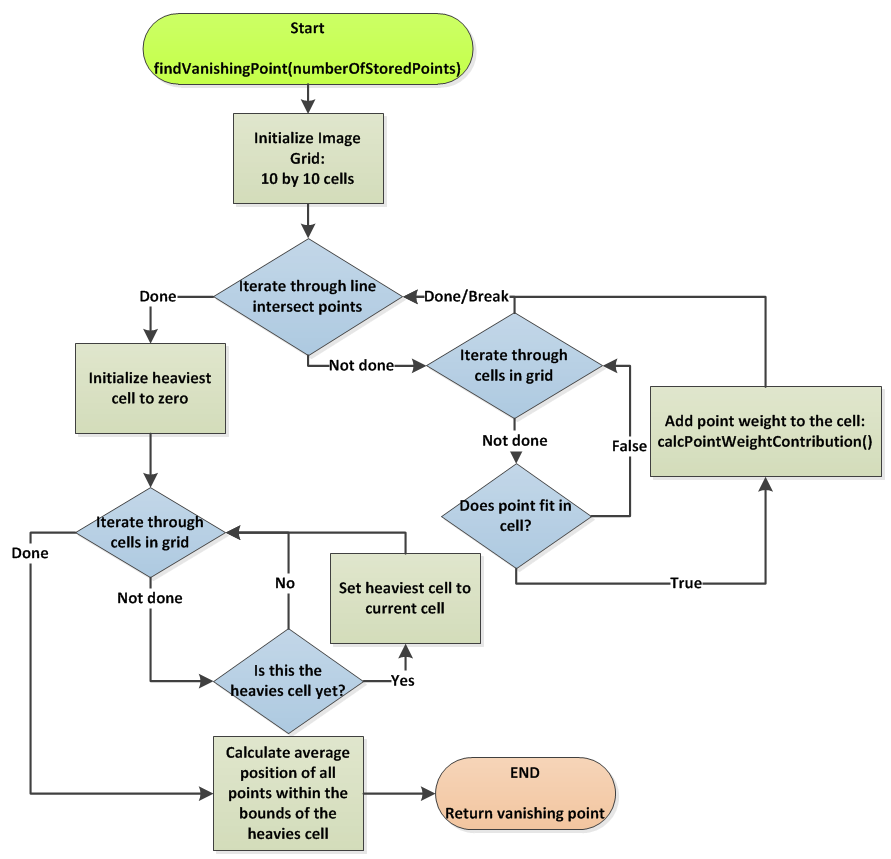
\includegraphics[scale=0.5]{findVp}
	\caption{Sequence diagram illustrating program execution when the user activates camera feed and VP detection.}
	\label{fig:findVp}
\end{figure}

\subsection{Vanishing Point Detector Application}

\paragraph{Program Structure}

The vanishing point detector was implemented as a QWidget Application in the Qt Creator IDE. The code excerpt shown in algorithm \ref{alg:edgelines} contains the most important image processing steps. A main thread, which may be called the GUI thread, handles all user related input and output. All image processing is done in the class "ImageProcessing" which inherits from QThread. This means that "ImageProcessing" controls a protected function "run()" which contains the threaded code and image processing steps. Figure \ref{fig:VpAppSequence} is a sequence diagram that shows the different classes and threads interact. The ellipse filter step is ommitted in the illustration; if it had been included, it would be called between "hough->detect()" and "getVanishingPoint()".

\begin{algorithm}[h]
	\caption{Vanishing point detector loop. Several lines of code are omitted in this example to make the processing more clear.}
	\label{alg:edgelines}
	\begin{verbatim}
	while(){
	    capture.read(cameraImg);
	    cvtColor(cameraImg,grayImg,CV_RGB2GRAY);
	    blur( grayImg, blurredImg, Size(3,3) );
	    Canny(blurredImg, edgesImg, lowerThresh, upperThresh, 3);
	    gpu_edgesImg.upload(edgesImg);
	    lines = detectHoughLines(gpu_edgesImg);   
	    newLines = mLineEllipseFilter.filterLines(lines,originalImage);
	    Point vanishingPoint = vpDetector.getVp(newLines,cameraImg);     
	}
	\end{verbatim}
\end{algorithm}

\begin{landscape}
	\begin{figure}
		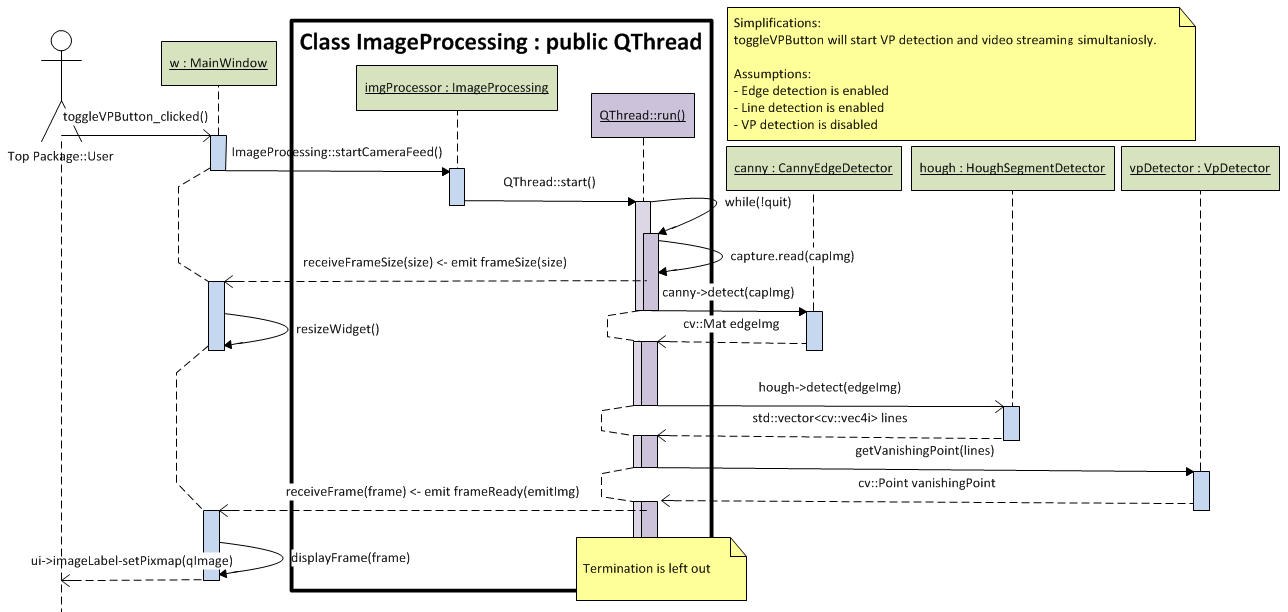
\includegraphics[scale=0.55]{VpAppSequence}
		\caption{Sequence diagram illustrating program execution when the user activates camera feed and VP detection.}
		\label{fig:VpAppSequence}
	\end{figure}
\end{landscape}



\paragraph{Graphical User Interface}

A graphical user interface was created so that the parameters for the canny edge detector and Hough lines detector could be tuned on-line. All widgets shown in figure \ref{fig:vpGui} have their functionality implemented. The user can turn on the camera feed, in this case from the web camera integrated into the laptop of the author, and switch line and edge detection on or off. Upper and lower edge detection thresholds, as well as line detection parameters can be set by using the sliders. The kernel size for the edge detector is set to 3 by 3, and can not be changed by the user. When both edge detection and line detection is enabled, the user may turn on the vanishing point detector module. In this particular application, the ellipse line filter module is not included.

\begin{figure}
	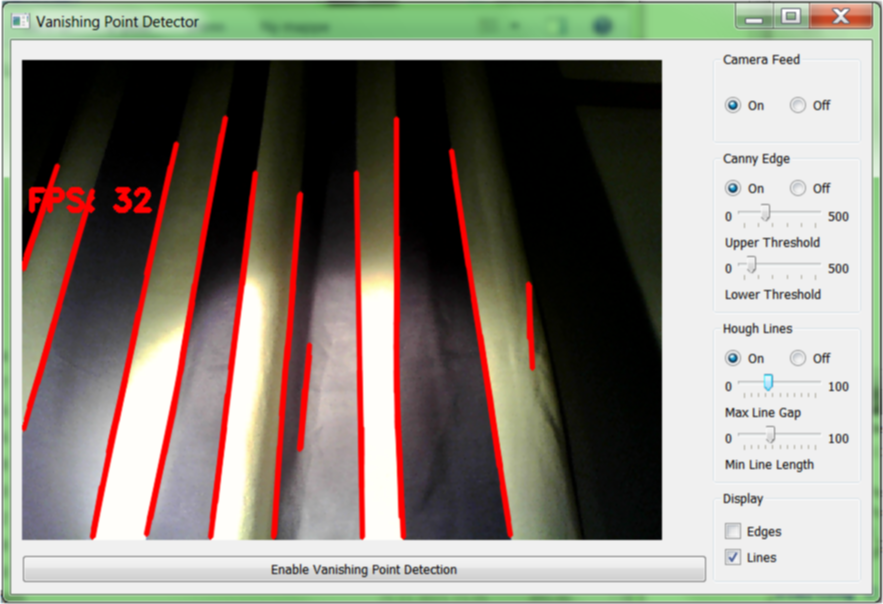
\includegraphics[scale=0.7]{VPGuiBlurred}
	\caption{Graphical user interface for the vanishing point detector. Note that the detected line segments are actually several lines overlapping each other.}
	\label{fig:vpGui}
\end{figure}

\subsection{Cause of Failure}

\section{Depth Perception and Obstruction Detection}

\subsection{Overview}

\subsection{The camera rig}

The two IP cameras were moved together to form a stereo camera. This stereo camera was used in two positions. The first camera position is on the pan-tilt module on the robot arm, see figure \ref{fig:rig_pantilt}. The second position is just over the LIDAR in front of the robot arm base, see figure \ref{fig:rig_front}.  The workshop at \gls{itk} made a mounting bracket, so that the cameras could be placed over the LIDAR. In stereo vision, it is essential that the positions of the cameras relative to each other is constant. One problem encountered throughout the project was that the camera assemby, when placed either at the pan-tilt module and over the LIDAR, was not rigid enough. The severity of this problem was somewhat alleviated by wrapping a strap around both the cameras. This camera rig is ad hoc, i.e. suitable for the purpose of this project, and a better solution should be used for succeeding projects.

\begin{figure}
	\centering
	\begin{subfigure}[b]{0.45\textwidth}
		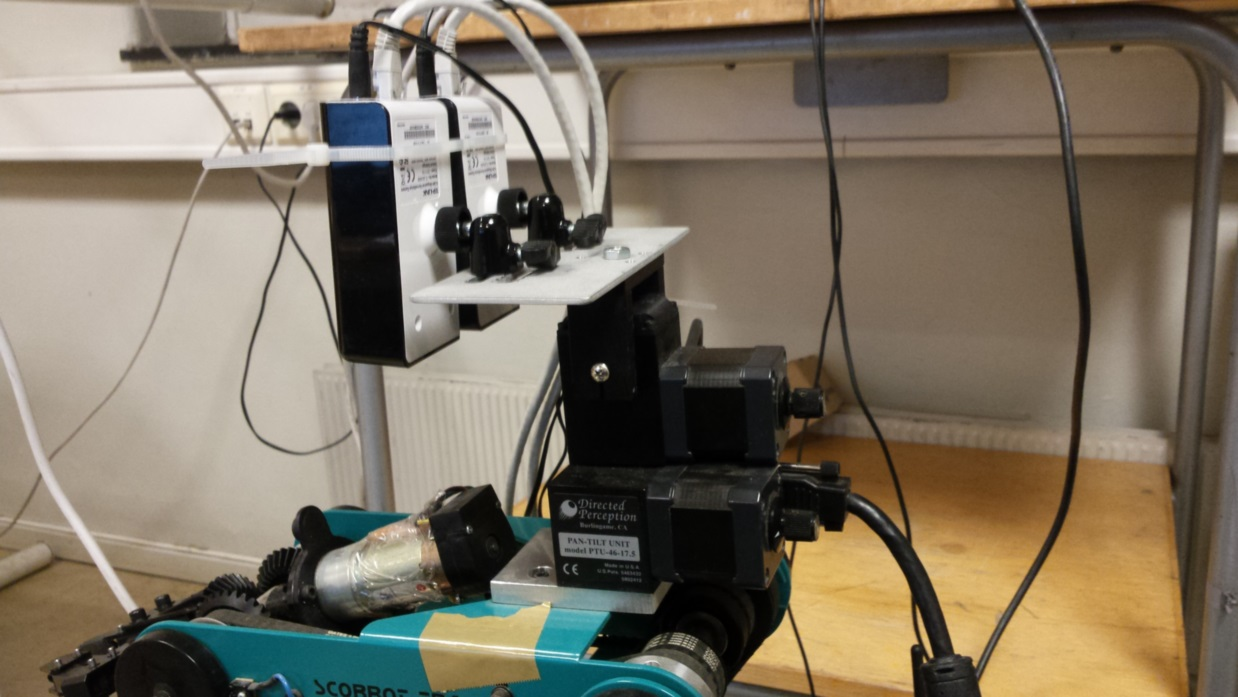
\includegraphics[width=\textwidth]{rig_pantilt}
		\caption{Camera pair mounted on the pan-tilt module.}
		\label{fig:rig_pantilt}
	\end{subfigure}
	\begin{subfigure}[b]{0.45\textwidth}
		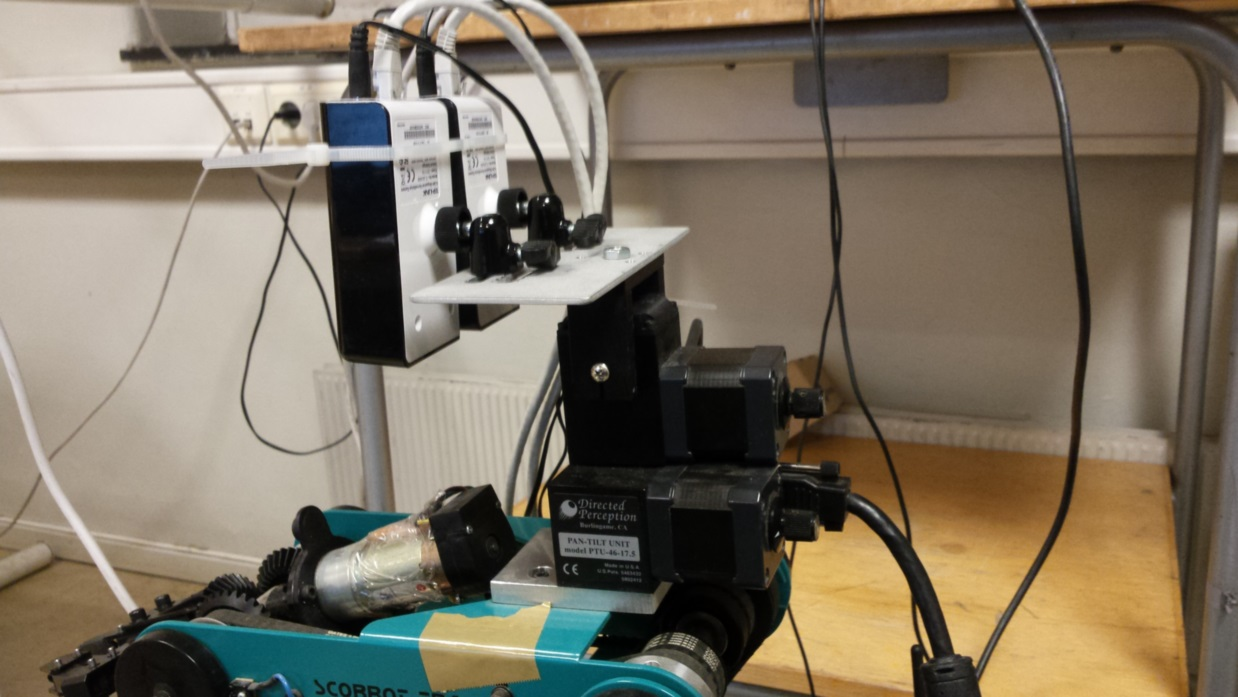
\includegraphics[width=\textwidth]{rig_pantilt}
		\caption{Camera pair mounted on the pan-tilt module.}
		\label{fig:rig_front}
	\end{subfigure}
	\caption{\label{fig:campos}The two camera positions.}
\end{figure}

\subsection{Graphical User Interface}

Tuning the parameters for stereo matching in OpenCV is a wearisome task, especially without a good graphical user interface. Figure \ref{fig:StereoGui} shows the user interface which was used to observe how parameter tuning alters the disparity map quality. Not all functionalities were implemented.

\begin{figure}
	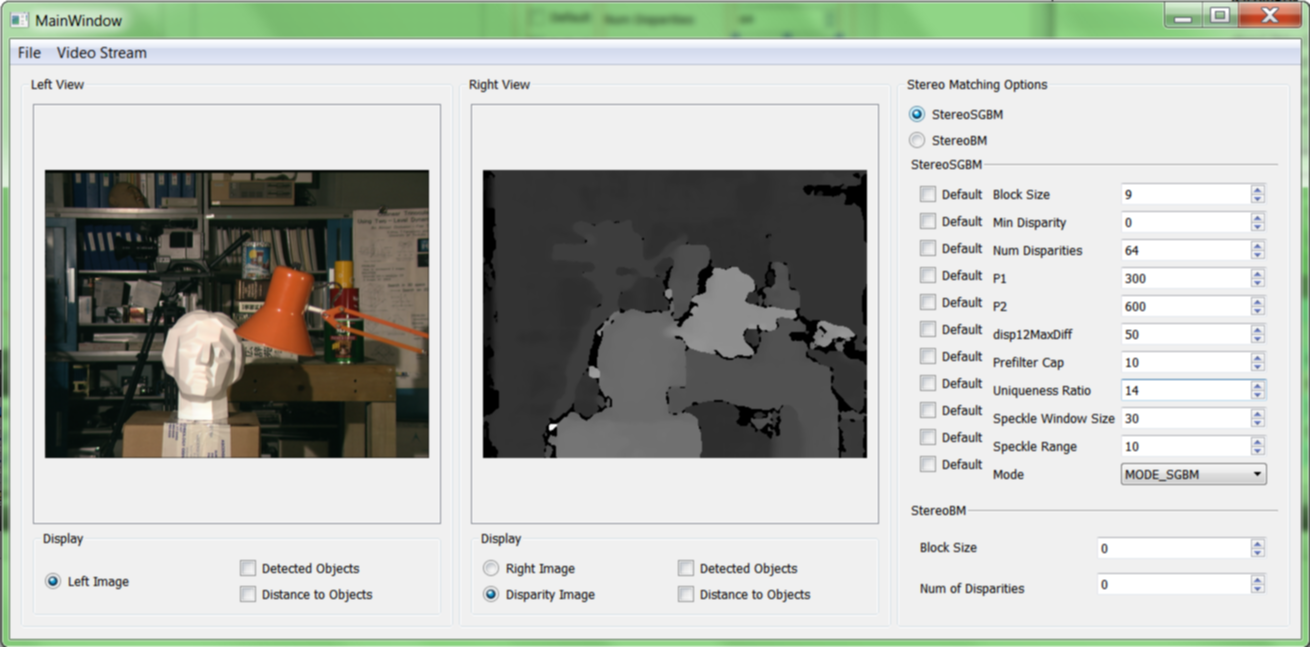
\includegraphics[scale=0.37]{StereoGui}
	\caption{Graphical user interface for stereo matching. A disparity map is computed from the Tsukuba samples by using StereoSGBM. }
	\label{fig:StereoGui}
\end{figure}

\subsection{Calibration}

As mentioned in chapter \ref{chp:theory}, all cameras will have some distortion. If the distortion is too severe, as it often will be in the context of stereo vision, the camera must be calibrated. In addition, it was assumed that the image planes were located on the same plane, and that a projection pair, for example the projections $X_L$ and $X_R$ of an object $X$, form two equal epipolar lines, $e_1$ and $e_2$, on the two image planes. In practice, these conditions are achieved through stereo calibration. The second purpose of the calibration procedure is to relate the sensor data to real world quantities, in order to measure the distance to detected objects. Code listings from Practical OpenCV by Samarth Brahmbhatt \cite{practicalopencv} has been used as a basis for calibration in this project. Some parts of his code is almost unchanged, while other parts of the listings are altered and expanded significantly. There are three steps in the calibration procedure:

\begin{enumerate}
	\item Single camera calibration: 
	\item Stereo calibration.
	\item Image rectification.
\end{enumerate}

See figure \ref{fig:calibproc} for an overview of the calibration procedure. All these steps require a familiar object with known dimensions to calibrate against. Among the three calibration patterns supported by OpenCV, this implementation utilized a black and white chessboard. The chessboard has 6 by 8 squares with sides $\approx 26 \, mm$ long.

\begin{figure}
	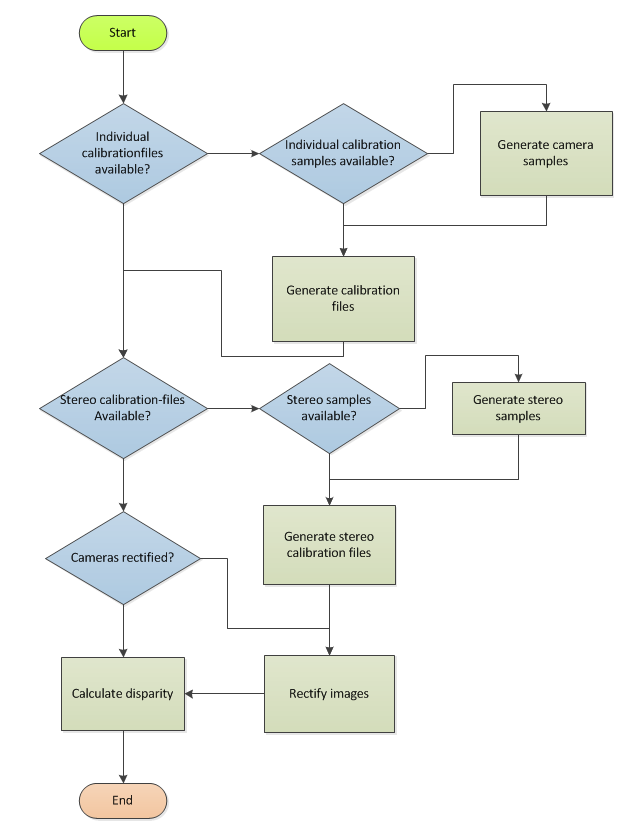
\includegraphics[scale=0.7]{StereoInit}
	\caption{An overview of the calibration procedure.}
	\label{fig:calibproc}
\end{figure}

\begin{figure}
	\centering
	\begin{subfigure}[b]{0.90\textwidth}
		
\includegraphics[width=\textwidth]{chess_pattern}
		\caption{The chessboard calibration pattern. The pattern was printed and taped to a flat surface.}
		\label{fig:chesspattern}
	\end{subfigure}
	\begin{subfigure}[b]{0.90\textwidth}
		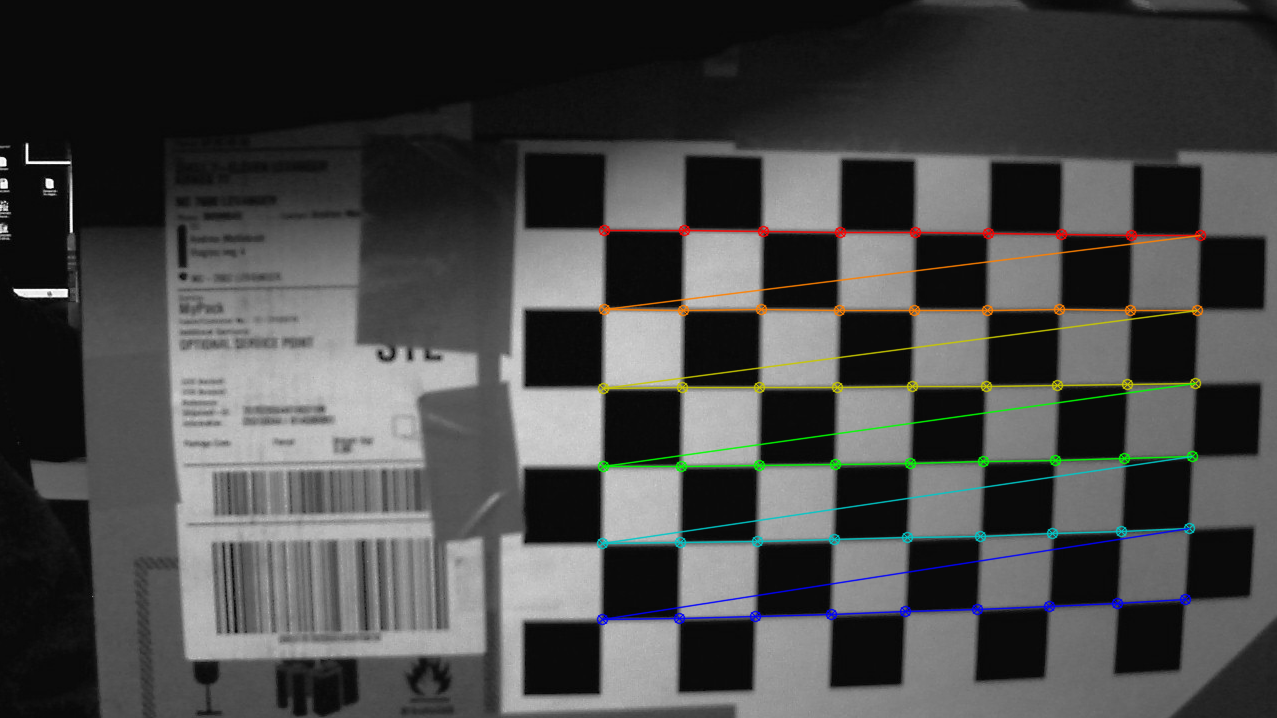
\includegraphics[width=\textwidth]{CamCalibDistorted}
		\caption{Chessboard detection. This is one of the sample images used to calibrate the camera. Notice the distortion in the lower right corner.}
		\label{fig:chessdetection}
	\end{subfigure}
	\caption{\label{fig:calibrationpattern}}
\end{figure}

\paragraph{Single Camera Calibration}

\begin{wrapfigure}{r}{0.48\textwidth}
	\vspace{-10pt} % Remove exessive whitespace
	\centering
	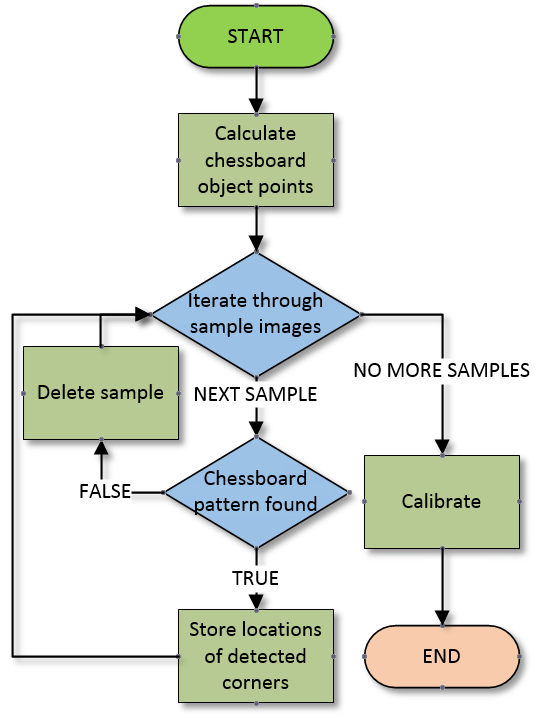
\includegraphics[width=0.50\textwidth]{singleCamCalib}
	\caption{\label{fig:singleCamCalib} Single camera calibration.}
	\vspace{-20pt} % Remove exessive whitespace
\end{wrapfigure}

In this step, the cameras are calibrated separately.  The purpose of this calibration procedure is to counter the constant radial and tangential distortion in a pinhole camera, and to identify the pinole camera model. The result of this procedure is the 3 by 3 camera matrix and the five distortion coefficients mentioned in the theory chapter. In the flowchart in figure \ref{fig:singleCamCalib}, assume that enough useful sample images are gathered and read into the program. In the last step, \gls{opencv}s calibration function will take inn the detected corners from the sample images and the chessboard dimentions. Finally, the calibration results are stored in an .xml file:

\begin{verbatim}
<?xml version="1.0"?>
<opencv_storage>
<cameraMatrix type_id="opencv-matrix">
  <rows>3</rows>
  <cols>3</cols>
  <dt>d</dt>
  <data>
    1.4478141049219482e+003 0. 6.6274484776761142e+002 
    0. 1.4432743079138295e+003 4.7609546427843065e+002 
    0. 0. 1.
  </data></cameraMatrix>
<distCoeffs type_id="opencv-matrix">
  <rows>1</rows>
  <cols>5</cols>
  <dt>d</dt>
  <data>
    -2.6128696949919589e-001 3.4600669963821584e-001
    -2.2331413545278616e-003 -2.5710895791919218e-003
    -3.7144316064113458e-001</data></distCoeffs>
</opencv_storage>
\end{verbatim}

\newpage

\begin{wrapfigure}{R}{0.4\textwidth}
\centering

	\begin{subfigure}[b]{0.35\textwidth}
        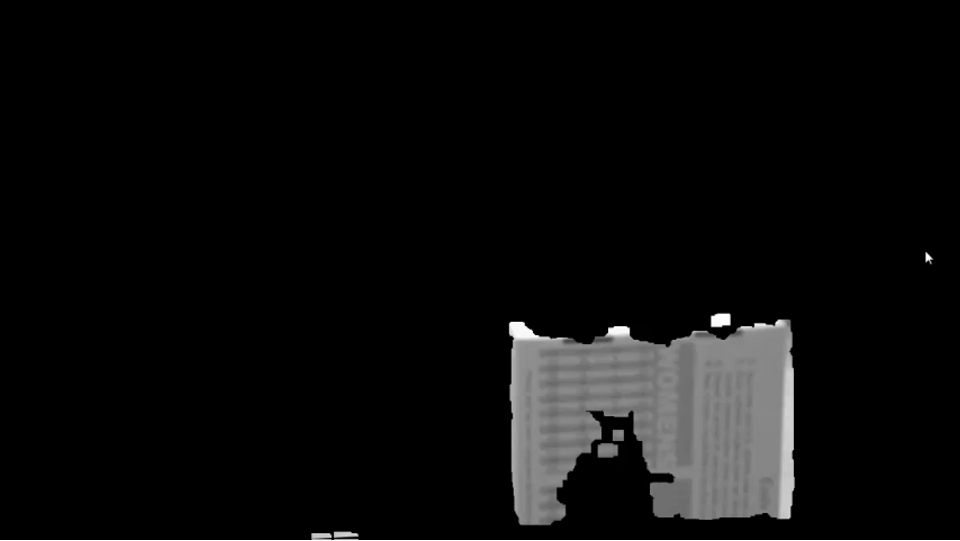
\includegraphics[width=\textwidth]{DepthLayer1}
	\end{subfigure}
	\par\medskip
	\begin{subfigure}[b]{0.35\textwidth}
        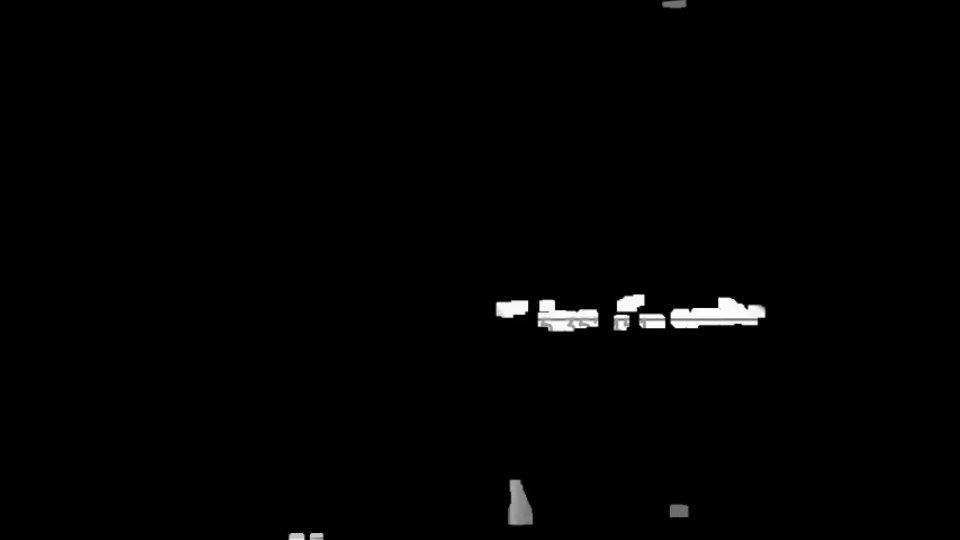
\includegraphics[width=\textwidth]{DepthLayer2}
	\end{subfigure}
	\par\medskip
	\begin{subfigure}[b]{0.35\textwidth}
        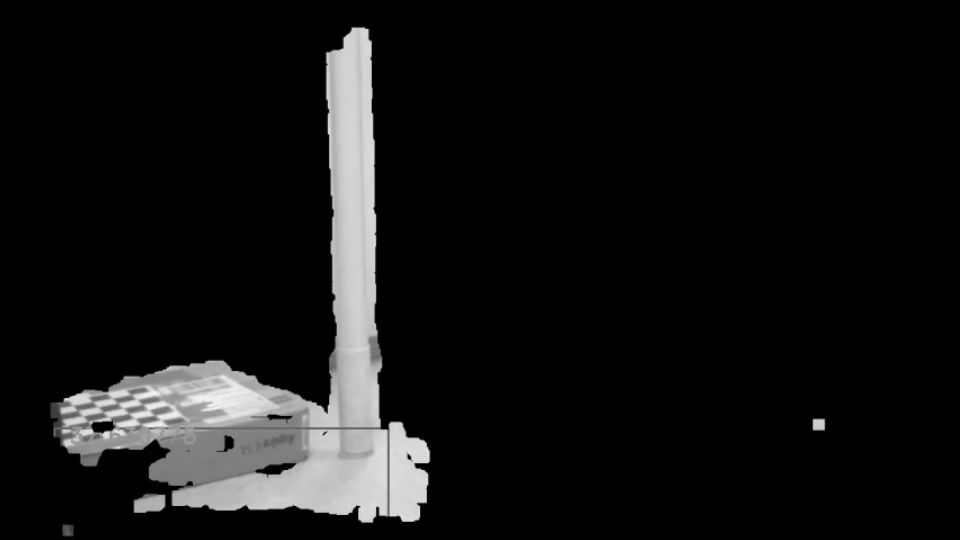
\includegraphics[width=\textwidth]{DepthLayer6}
	\end{subfigure}
	\par\medskip
	\begin{subfigure}[b]{0.35\textwidth}
        
\includegraphics[width=\textwidth]{DepthLayer7}
	\end{subfigure}
	\par\medskip
	\begin{subfigure}[b]{0.35\textwidth}
        
\includegraphics[width=\textwidth]{DepthLayer8}
	\end{subfigure}
	
\caption{Some of the depth layers in figure \ref{fig:StereoMatching} separated by color filtering. The top image is the closest layer, while the most distant layer is at the bottom.}
\label{fig:layers2}
\end{wrapfigure}

When all the image samples has been read into the program, the program will check if the chessboard can be detected. If the chessboard is present in the image, the position of the corners will be stored in  

\paragraph{Stereo Calibration}

Stereo calibration is almost exactly the same as single camera calibration. An important difference is obviously that sample images must be taken from both cameras simultaniously. The calibration pattern must be detectable in both frames. Stereo calibration will generate a new set of data:

\begin{description}
	\item[R: ] 3 by 3 rotation matrix between the two cameras.
	\item[T: ] Translation between the two cameras. Denoted $B$ in the theory chapter. Relates the left camera to the right together with $R$. 
	\item[E: ] 3 by 3 essential matrix.
	\item[F: ] 3 by 3 fundamental matrix.
\end{description}

These matrices will be stored in a new file ''stereo\_calib.xml'' together with the distortion coefficients and camera matrices from the two single camera calibrations. These values will be applied in the next calibration step.

\paragraph{Stereo Rectification}

Rectification is the final step before stereo matching can be performed. In this step, the information that is necessary to align the stereo frames. When the frames are aligned, Rectification is completed by:

\begin{enumerate}
	\item Loading ''stereo\_calib.xml'' and reading in the camera matrices, distortion coefficients, $R$ and $T$.
	\item Calling ''stereoRectify()'' with the data above as input.
\end{enumerate}

 ''stereoRectify()'' will write data unto a set of new matrices:

\begin{description}
	\item[Rl: ] 3 by 3 rotation matrix between the two cameras.
	\item[Rr: ] Translation between the two cameras. Denoted $B$ in the theory chapter. Relates the left camera to the right together with $R$. 
	\item[Pl: ] 3 by 3 essential matrix.
	\item[Pr: ] 3 by 3 fundamental matrix.
	\item[Q: ] 3 by 3 fundamental matrix.

\end{description}

%\begin{figure}
%\includegraphics[scale=•]{•}
%\end{figure}

\subsection{Stereo Matching}

\begin{figure}
\centering
 \begin{subfigure}[b]{0.45\textwidth}
        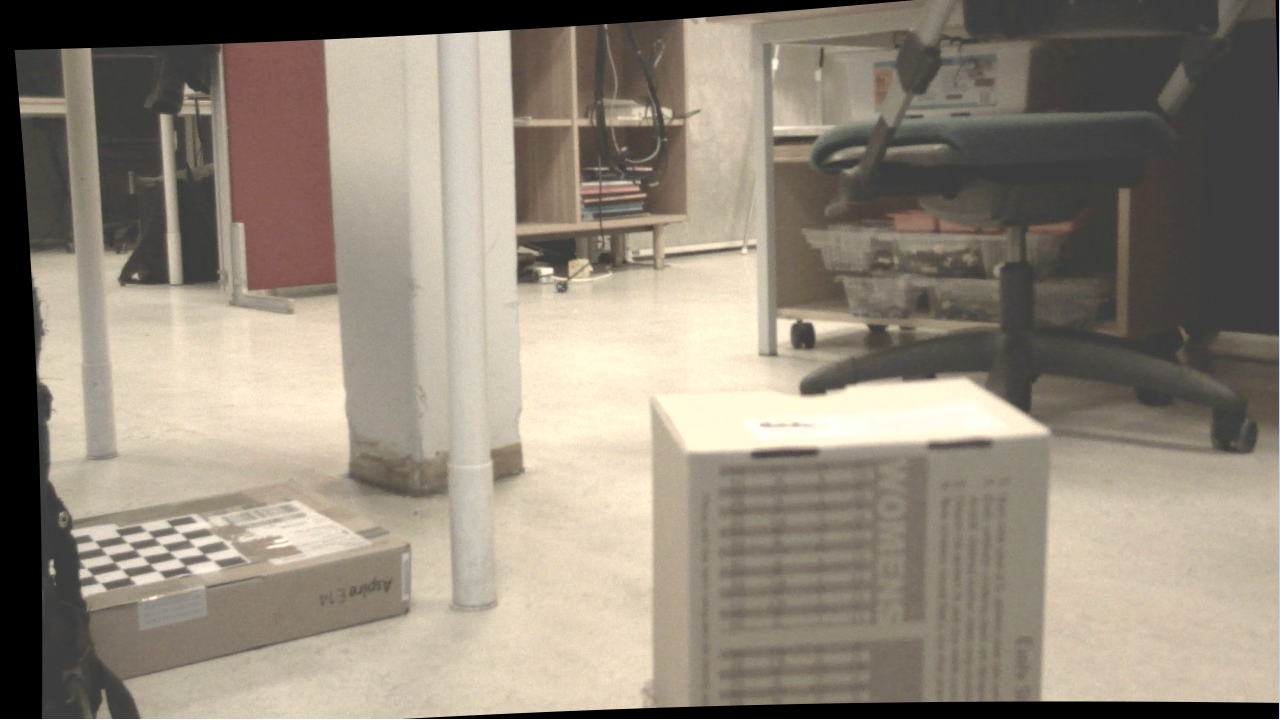
\includegraphics[width=\textwidth]{OriginalExample}
        \caption{Left camera image.}
        \label{fig:OriginalExample}
    \end{subfigure}
    \begin{subfigure}[b]{0.45\textwidth}
        
\includegraphics[width=\textwidth]{DispExample}
        \caption{Disparity map.}
        \label{fig:DispExample}
    \end{subfigure}
    \caption{\label{fig:StereoMatching}The result of StereoSGBM.}
\end{figure}

\subsection{Finding Obstructions}

\begin{figure}
	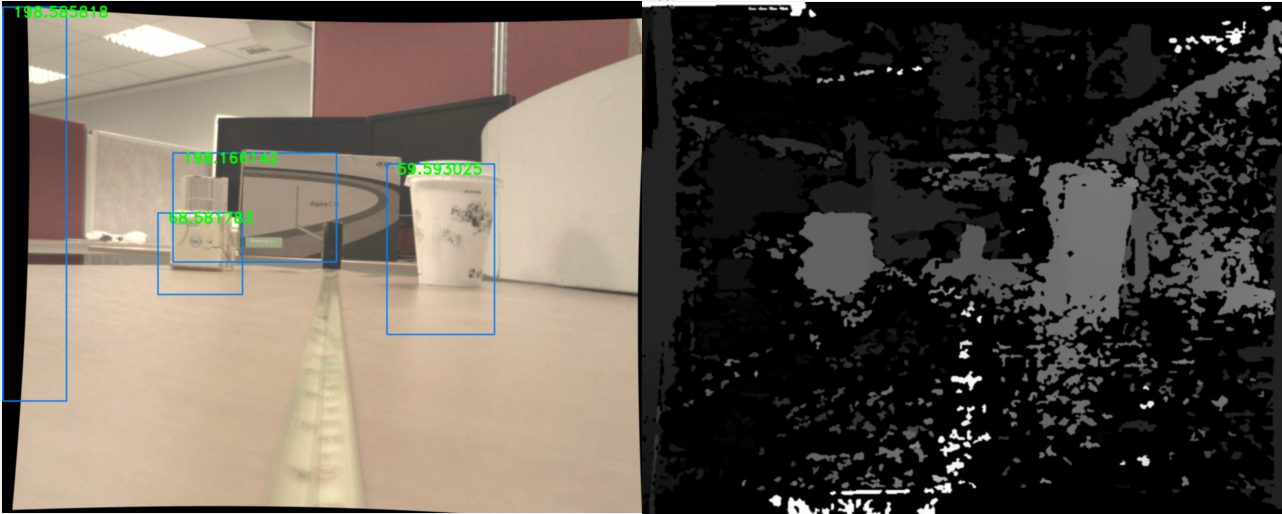
\includegraphics[scale=0.37]{obstruction}
	\caption{Dummy text. }
	\label{fig:obstruction}
\end{figure}

\subsection{Distance Measurment}

\subsection{Problems Encountered During Implementation }

\renewcommand*{\bibname}{References}
\bibliographystyle{alpha}
\bibliography{main}

% Uncomment the following if you have any appendix
 \appendix
 \addtocontents{toc}{%
  \protect\vspace{1em}% 
  \protect\noindent \bfseries \appendixtocname\protect\par
  \protect\vspace{-.5em}%
 }
 \renewcommand{\chaptername}{\appendixname}
%% include below possible appendices (chapters)



\end{document} 
